\documentclass[11pt]{beamer}
\usetheme{Madrid}
\usepackage[utf8]{inputenc}
\usepackage[english,german]{babel}
\usepackage[T1]{fontenc}
\usepackage{amsmath}
\usepackage{amsfonts}
\usepackage{amssymb}
\usepackage{graphicx}
\usepackage[style=authortitle-icomp,backend=biber]{biblatex}
\usepackage[babel,german=guillemets]{csquotes}
\addbibresource{seminararbeit_monitoring.bib}
\author{Markus Österle}
\title{Servermonitoring im Rechenzentrum}
%\setbeamercovered{transparent} 
%\setbeamertemplate{navigation symbols}{} 
%\logo{} 
%\institute{} 
\date{18. Januar 2016} 
\subject{Präsentation zur Seminararbeit im Studiengang \glqq Verwaltungsinformatik\grqq} 
\begin{document}
\begin{frame}
\titlepage
\end{frame}

%\begin{frame}
%\tableofcontents
%\end{frame}

\begin{frame}{Übersicht - roter Faden}
\begin{itemize}
	\item Monitoring was ist das eigentlich? - Definitionen
	\item Warum Monitoring?
	\item Wie wird es gemacht? - verwendete Software
\end{itemize}
\end{frame}
\begin{frame}{Monitoring}
	%TODO: Hier lt. Duden oder korrektes Zitat?
	Laut \cite[S. 701; Stichwort Monitoring]{duden}: \\
	
	\begin{center}
		\glqq [Dauer]beobachtung (eines bestehenden Systems)\grqq
	\end{center}
	
\end{frame}
\begin{frame}{Arten des Monitorings}
	\begin{itemize}
		\item proaktives Monitoring
		\item reaktives Monitoring
		\item SLA Monitoring
	\end{itemize}
\end{frame}
%TODO Warum Monitoring hier oder unten?
\begin{frame}{Proaktives Monitoring}
	\begin{center}
		Monitoring, bei dem versucht wird, Event-Muster zu ermitteln, um mögliche zukünftige Ausfälle zu prognostizieren.
	\end{center}
	 
\end{frame}
\begin{frame}{Reaktives Monitoring}
	\begin{center}
		Monitoring, das als Reaktion auf ein bestimmtes Event entsprechende Maßnahmen einleitet. Beispielsweise die Auslösung eines Batchjobs, sobald ein vorheriger Batchjob abgeschlossen wurde, oder die Erfassung eines Incident, wenn ein Fehler auftritt. 
	\end{center}
\end{frame}
\begin{frame}{SLA Monitoring}
	Definition SLA \\
	Definition SLA Monitoring
\end{frame}
\begin{frame}{Warum Monitoring?}
	content...
\end{frame}
\begin{frame}{Nagios Historie}

\end{frame}
\begin{frame}{Nagios - Aufbau}
	%TODO Aktive/Passive Checks was ist das...
	\begin{figure}
		\centering
		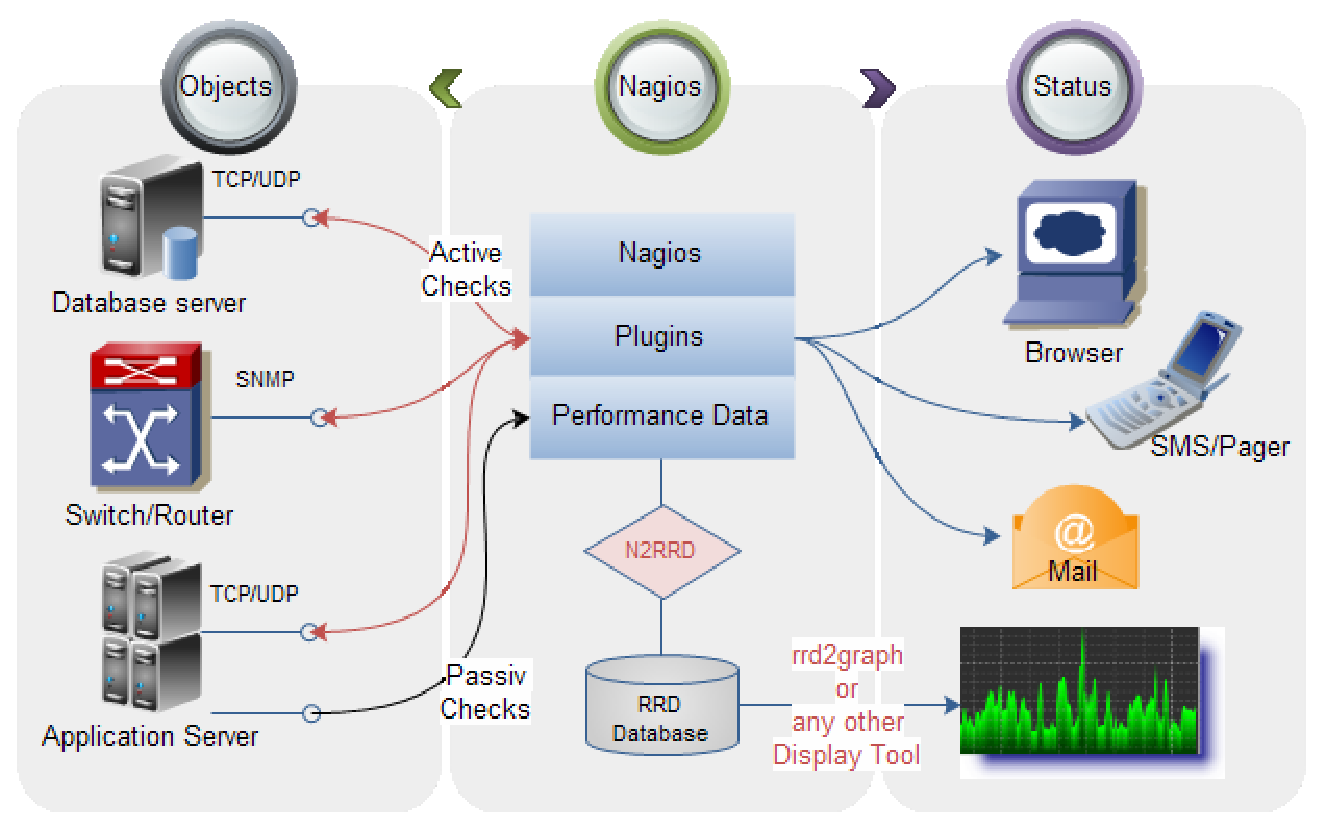
\includegraphics[width=0.9\textwidth]{pics/NagiosMonitoring.eps}
		\caption[Grober Aufbau von Nagios]{Aufbau einer Nagios Appliance - Quelle: \textcite{nagiosaufbau}}
	\end{figure}
\end{frame}
\begin{frame}{Nagios - Probleme}
	content...
\end{frame}
\begin{frame}{Check\_MK - die Lösung}
	%TODO Check_MK Screenshot
\end{frame}
\begin{frame}{Check\_MK - Aufbau}
	\begin{figure}
		\centering
		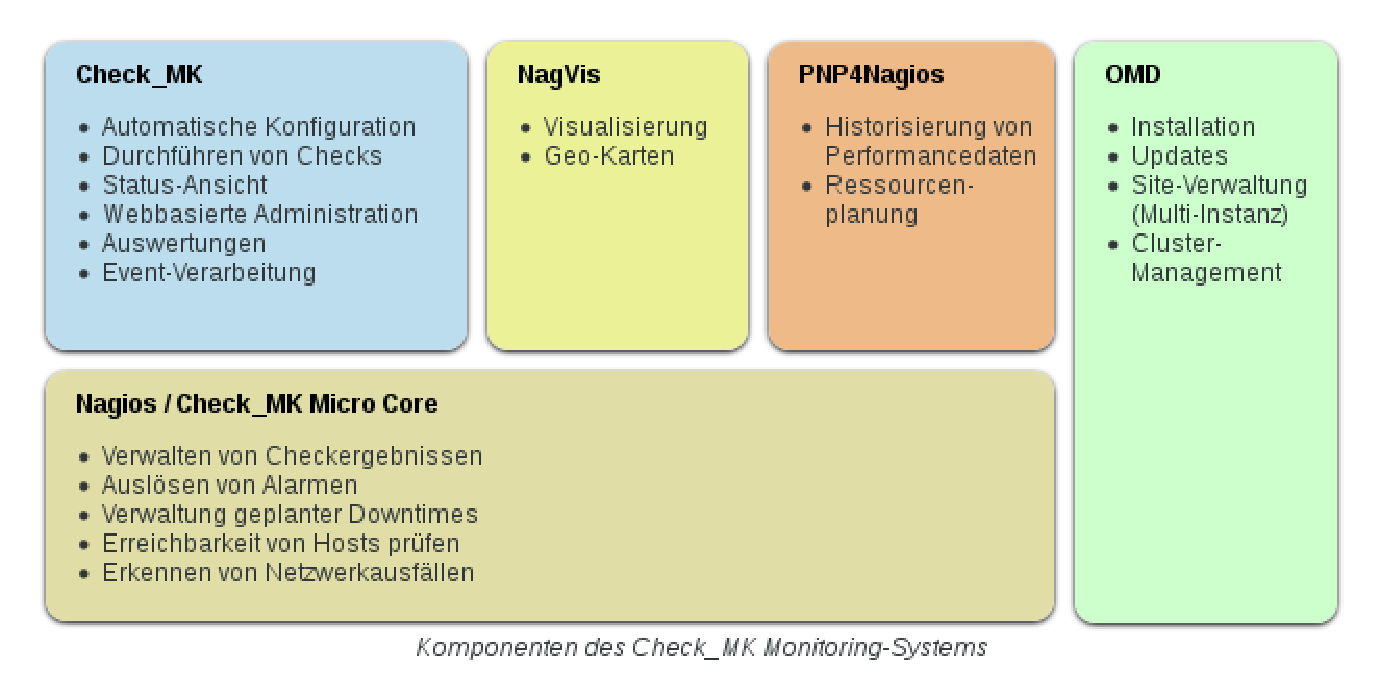
\includegraphics[width=1\textwidth]{pics/checkMKAufbau.eps}
		\caption[Komponenten des Check\_MK Monitoring Systems]{Komponenten des Check\_MK Monitoring Systems (Quelle: \textcite{checkmkmonitoringpic})}
	\end{figure}
\end{frame}
\begin{frame}{Fürs Protokoll: Ein Elch - Elasticsearch - Logstash - Kibana}
\begin{itemize}
	\item Elasticsearch
	\item Logstash
	\item Kibana
\end{itemize}
\end{frame}
\begin{frame}{Quellen}
	\printbibliography
\end{frame}
\end{document}